\documentclass[10pt,letterpaper]{article}
\usepackage[margin=0.75in,headheight=14pt]{geometry}
\usepackage[T1]{fontenc}
\usepackage{lmodern}
\usepackage{microtype}
\usepackage{amsmath,amssymb,amsthm,mathtools}
\usepackage{booktabs,tabularx,array}
\usepackage{multicol}
\usepackage{enumitem}
\usepackage{xcolor}
\usepackage[hidelinks]{hyperref}
\usepackage{tikz}
\usetikzlibrary{arrows.meta,positioning,shapes.geometric}
\usepackage{caption}
\usepackage{fancyhdr}
\usepackage{listings}
\definecolor{navy}{HTML}{17334D}
\definecolor{muted}{HTML}{566575}
\definecolor{pale}{HTML}{EFF3F6}
\hypersetup{pdftitle={When Do Specialized Expert Models Beat Monolithic LLMs?},pdfauthor={Kenneth Hurley},pdfsubject={Genius Cognitive System technical working paper}}
\pagestyle{fancy}
\fancyhf{}
\fancyhead[L]{\footnotesize\color{muted}GCS / Specialist-Hybrid Research Draft}
\fancyhead[R]{\footnotesize\color{muted}WIP --- Unpublished}
\fancyfoot[C]{\footnotesize\thepage}
\setlength{\columnsep}{0.27in}
\setlength{\parindent}{0.85em}
\setlength{\parskip}{0.1em}
\setlist[itemize]{leftmargin=1.25em,topsep=3pt,itemsep=1pt}
\setlist[enumerate]{leftmargin=1.3em,topsep=3pt,itemsep=2pt}
\newtheorem{proposition}{Proposition}
\newcommand{\GCS}{\textsc{GCS}}
\newcommand{\ELM}{\textsc{ELM}}
\newcommand{\EJM}{\textsc{EJM}}
\newcommand{\NTP}{\textsc{NTP}}
\newcommand{\expect}{\mathbb{E}}
\newcommand{\code}[1]{\texttt{#1}}
\newcommand{\status}[1]{\textcolor{navy}{\textbf{#1}}}
\begin{document}
\begin{center}
{\large\bfseries\color{navy} When Do Specialized Expert Models Beat Monolithic LLMs?}\\[5pt]
{\normalsize\bfseries A Testable Hybrid Architecture for the Genius Cognitive System, Informed by Good-View Joint-Embedding Predictive Learning}\\[10pt]
{\small Kenneth Hurley}\\[2pt]
{\small Genius Ventures / Genius Cognitive System}\\[4pt]
{\footnotesize November 2, 2026 \quad $\cdot$ \quad \textbf{Working draft v0.1} \quad $\cdot$ \quad \textbf{Not submitted or published}}\\[9pt]
\begin{minipage}{0.94\textwidth}
\small
\noindent\textbf{Abstract.} Large language models (LLMs) can solve many tasks, but their parameter count alone does not show that a single model is the best choice for every request. The Genius Cognitive System (GCS) proposes a semantic core, routed Expert Language Models (ELMs), bounded Expert Judgment Models (EJMs), grounding, selective checking, and local or distributed execution. This paper presents a falsifiable claim: for a defined mixture of tasks and a fixed quality target, a well-routed specialist system can reduce measured inference cost and latency while preserving or improving task success relative to a fixed general-model baseline. We connect this claim to Balestriero and LeCun's 2026 theoretical and empirical work on good-view Joint-Embedding Predictive Architectures (JEPAs), which establishes conditional representation-alignment results and reports a strong advantage on cross-modal alignment. We do not infer that JEPA alignment establishes the superiority of GCS or of ELMs on general reasoning. Instead, we propose an optional good-view alignment component, a formal decision and checking model, matched baselines, preregistered tests, and explicit conditions for a future proof or a narrower empirical conclusion. Current source evidence supports a partial router/ELM prototype; full integrated GCS claims and all outcome comparisons remain unverified.
\\[4pt]
\noindent\textbf{Keywords:} specialist language models; routing; joint embeddings; JEPA; semantic alignment; verification; inference cost; distributed inference; GCS.
\end{minipage}
\end{center}
\vspace{7pt}
\noindent\colorbox{pale}{\parbox{\dimexpr\textwidth-2\fboxsep\relax}{\footnotesize\textbf{Evidence status.} This document is a design and evaluation plan. It contains derived conditional statements, not experimental proof that GCS outperforms any LLM. All GCS performance tables intentionally contain no fabricated results. Keep it private until code, data, tests, and review are complete.}}
\vspace{10pt}
\begin{multicols}{2}
\section{Question and central hypothesis}
For a task distribution $\mathcal{D}$, compare a fixed general-purpose LLM $L$ with a hybrid policy $H$ that chooses whether to use a semantic core, a domain expert, a bounded judge, grounding, a verifier, or a fallback. The meaningful claim is \emph{conditional superiority}: does the hybrid reach at least the same verified task success, at lower resource cost, under the same service constraints?

We make three claims, each with a different evidence burden.
\begin{enumerate}
\item \textbf{Architecture claim:} specialization can avoid running a large general-purpose model on tasks that compact models solve reliably. This is a design claim.
\item \textbf{Training claim:} when different specialists need to share a semantic reference, carefully chosen positive views may improve the alignment of their representations. This is motivated by JEPA research, subject to its assumptions.
\item \textbf{System claim:} a complete GCS hybrid can improve task success, latency, and cost compared with one or more monolithic baselines. This is a \emph{hypothesis awaiting measurement}, not a result.
\end{enumerate}

A model can use fewer parameters and still be slower end-to-end when its route includes retrieval, several experts, or remote work. Accordingly, model size is not our optimization target. Measured success per unit cost, with explicit latency and safety constraints, is.

\section{What the JEPA paper establishes}
Balestriero and LeCun's \emph{Proving and Improving the Platonic Representation Hypothesis with JEPAs} \cite{balestriero2026} starts from a finite world state $z$, separate observations in different modalities, and positive pairs drawn from world-state relations. Its Theorem 1 shows equality of learned embeddings \emph{up to an orthogonal rotation}, given a common positive-pair distribution and minimizers unique up to rotation. The spectral form assumes centered, whitened embeddings with an eigengap. Its Theorem 2 bounds residual misalignment when the positive-pair kernels differ. Its treatment of next-token prediction as a bad-view JEPA is a structural analogy, with qualifications made explicit by the authors.

The experiments reported in that paper find that a 109M-parameter good-view text JEPA reaches 0.184 mutual 10-nearest-neighbor alignment with DINOv2 on WIT-1024, versus 0.154 for Qwen2.5-72B and 0.151 for Llama-3-70B under the reported protocol. With the same corpus and encoder family, a good-view JEPA reaches comparable alignment with 21.6M training samples where next-token prediction needs about 900M samples: approximately $42\times$ fewer samples, for \emph{that alignment target}. These numbers belong to the source paper, not GCS.

The distinction is vital: \emph{cross-modal representational agreement is not proof of answer correctness, broad reasoning skill, energy savings, cost reduction, or superiority on arbitrary tasks}. The source paper also names limits: idealized injective observations, matched marginals and spectral assumptions, reliance on recaptioned texts, and imperfect correspondence between theory and deployed training procedures \cite{balestriero2026}.

\subsection{The part GCS might use}
GCS needs expert outputs and evidence to refer to the same facts, constraints, entities, and requested outcomes. A useful \emph{proposed} JEPA component would align compact representations of several observations of the same task state, while making them insensitive to surface form. Examples include two independent explanations of a verified program behavior, two descriptions of one observed event, or a trace and a structured result record that describe the same measured operation. A positive pair must come from the \emph{same verified world state}; two paraphrases of a mistaken answer are not good evidence.

\section{The GCS architecture under study}
GCS documents define the semantic and policy contracts; GNUS-NEO-SWARM is assigned the RuntimeCoordinator; MNN owns tokenizer/model execution; SGProcessingManager owns declared processing workloads; SuperGenius owns distributed worker selection and settlement \cite{gcsadr}. These boundaries prevent the cognitive planner from being confused with the model runtime or the peer scheduler.

The proposed composition has four parts:
\begin{enumerate}
\item \textbf{Semantic Core:} a general backbone for broad tasks and fallback generation.
\item \textbf{Specialist capabilities:} ELMs for language generation and transformation; EJMs for bounded judgments; optionally other processor kinds (including diffusion-based refinement) \cite{gcsrouter}.
\item \textbf{Cognitive control:} feature extraction, selection, typed execution plans, budgets and selective checking; memory and grounding only under the configured policy.
\item \textbf{Execution:} local/private runtime first when allowed; distributed jobs through the SuperGenius processing layer when needed.
\end{enumerate}

\begin{center}
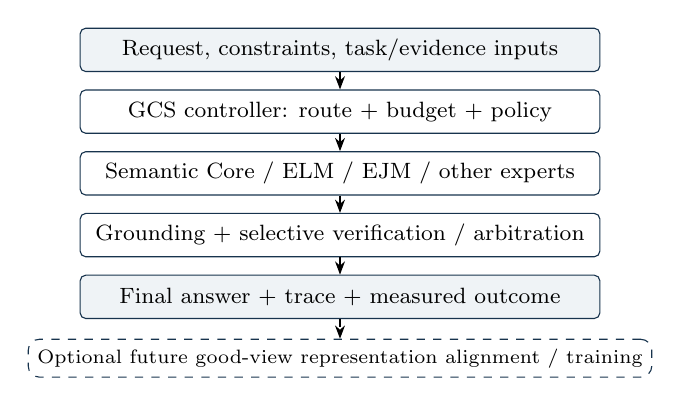
\begin{tikzpicture}[>=Stealth, node distance=0.22cm, every node/.style={font=\footnotesize}]
\tikzstyle{b}=[draw=navy,rounded corners=2pt,align=center,minimum width=6.6cm,minimum height=0.55cm,fill=white]
\node[b,fill=pale] (a) {Request, constraints, task/evidence inputs};
\node[b,below=of a] (r) {GCS controller: route + budget + policy};
\node[b,below=of r] (e) {Semantic Core / ELM / EJM / other experts};
\node[b,below=of e] (v) {Grounding + selective verification / arbitration};
\node[b,below=of v,fill=pale] (s) {Final answer + trace + measured outcome};
\draw[->] (a) -- (r);\draw[->] (r) -- (e);\draw[->] (e) -- (v);\draw[->] (v) -- (s);
\node[draw=navy,dashed,rounded corners,align=center,font=\scriptsize,minimum width=6.6cm,below=0.25cm of s] (f) {Optional future good-view representation alignment / training};
\draw[->,dashed] (s) -- (f);
\end{tikzpicture}
\captionof{figure}{Conceptual GCS path. The dashed JEPA component is a research proposal, not a verified integration. Distributed execution is conditional, not mandatory for each request.}
\end{center}

\subsection{Code evidence, not production proof}
We inspected public source at GCS commit \code{6d05e857} and GNUS-NEO-SWARM commit \code{1253ceae} (November 2, 2026). In NEO-SWARM, \code{rule\_based\_router.cpp} selects SingleNode, Specialist or Swarm based on prompt features. \code{elm\_chain\_builder.cpp} specifies chains such as Math $\to$ Verifier, Grounding $\to$ Draft $\to$ Verify, and Planner $\to$ Draft $\to$ Verify $\to$ Refine. \code{domain\_elm.cpp} chooses a dedicated model engine or a shared-backbone fallback. Tests exist for router features, targets, and execution chains \cite{neoswarmrouter,neoswarmchain,neoswarmdomain}.

Those tests show that certain source paths are implemented. They do not show that specialized models have been trained, that the full chain was benchmarked, or that the complete governed memory/verification pipeline is live. The GCS implementation register expressly treats the full system as planned or partial and states that no certified production benchmark has been published \cite{gcsstatus,gcsbench}.

\section{A formal task and routing model}
Let $x\sim\mathcal D$ be a task with an objectively scored target. Let $\mathcal A$ be available execution plans: a general model, core-only, one specialist, multi-specialist, and verified variants. For each plan $a$, let
\begin{align}
q_a(x)&=\Pr(\text{accepted answer is correct}\mid x,a),\\
c_a(x)&=\text{measured money / energy / work cost},\\
t_a(x)&=\text{end-to-end elapsed time},\\
r_a(x)&=\text{policy or safety risk}.
\end{align}
A routing policy $\pi(x)$ selects a plan from $\mathcal A$. Define measured system quality and cost
\begin{equation}
Q(\pi)=\expect_{x\sim\mathcal D}[q_{\pi(x)}(x)],\qquad
C(\pi)=\expect_{x\sim\mathcal D}[c_{\pi(x)}(x)].
\label{eq:quality}
\end{equation}
We call the hybrid \emph{superior on a defined benchmark} only if it satisfies a declared quality non-inferiority threshold $Q(H)\ge Q(L)-\epsilon$ and simultaneously achieves a specified gain, such as $C(H)<C(L)$ with acceptable $p95$ latency, or strictly improves quality without exceeding budget. We will also report each metric on its own; a scalar score must not hide poor safety or tail latency.

\subsection{Conditional routing bound}
\begin{proposition}[Router regret under bounded losses]
Let $\ell_a(x)\in[0,R]$ be the complete measured loss of plan $a$, including a chosen quality/cost trade-off. Assume an oracle $a^*(x)$ minimizes $\ell_a(x)$ for each task. If a router chooses a plan different from the oracle on a fraction $\eta$ of tasks, then
\begin{equation}
0\le\expect[\ell_{\pi(x)}(x)-\ell_{a^*(x)}(x)]\le\eta R.
\end{equation}
\end{proposition}
\noindent\emph{Derivation.} On correctly routed tasks regret is zero. Elsewhere it lies between zero and $R$; taking the expectation gives the bound. This says nothing about the actual $\eta$, the usefulness of an oracle, or whether the hybrid beats $L$. Those require measurement.

\subsection{Conditional checking benefit}
\begin{proposition}[One checker and fallback]
Suppose the first candidate is wrong with probability $e$; a checker detects a wrong answer with probability $d$ and falsely rejects a correct answer with probability $f$. Rejected answers go to a fallback that is correct with conditional probability $q_f$. Under this simplified, task-averaged model,
\begin{equation}
Q_{\mathrm{check}}=(1-e)(1-f)+q_f[(1-e)f+ed].
\end{equation}
Checking improves success over the initial $1-e$ exactly when
\begin{equation}
edq_f>(1-e)f(1-q_f).
\end{equation}
\end{proposition}
\noindent\emph{Derivation.} Sum the probability of accepting an originally correct answer and obtaining a correct fallback after rejection, then subtract $1-e$. The condition shows why \emph{verification by itself is not a guarantee}: a weak checker or fallback may lower quality. Conditional estimates $e,d,f,q_f$ must be measured by task class.

\subsection{True cost of a hybrid}
For a task with chosen steps $S(x)$, total system cost is
\begin{equation}
C_H(x)=C_{\rm route}+C_{\rm core}+\sum_{j\in S(x)}C_j+C_{\rm check}+C_{\rm retrieval}+C_{\rm network}.
\label{eq:cost}
\end{equation}
If a step is skipped its cost is zero. A cheaper specialist yields an end-to-end saving only when avoided general-model work exceeds all extra steps and their overhead. In distributed mode, retries, serialization and settlement belong in the measured total.

\section{JEPA-inspired representations for GCS}
\subsection{Positive views tied to evidence}
The source theorem applies to separately learned representations of modalities that see the same underlying world states, with suitable positive-pair distributions. It does \emph{not} assert that independently distilled ELMs, autoregressive generators, or GCS routes will align automatically. We therefore propose a new, optional representation stage with a documented bridge between the source assumptions and our setting:
\begin{enumerate}
\item Identify a verified state $z$: e.g., a unit-tested program behavior, an attributed document fact, or a replayed tool outcome. Assign stable state and source IDs.
\item Form independent positive observations $v_1(z),v_2(z)$ that preserve the same relevant fact. Exclude pairs that merely repeat wording or share an unsupported claim.
\item Train a compact encoder $f_m$ using good-view positives, an anti-collapse loss and a documented embedding dimension. Use the source paper's objective as a comparator; do not claim theoretical coverage of arbitrary GCS heads.
\item Estimate cross-expert alignment through mutual $k$-NN, centered kernel alignment, and orthogonal Procrustes on held-out states. Track false-positive pairs and privacy boundaries.
\item Only after successful alignment and task tests, add the embeddings to routing, memory retrieval, evidence linking, or specialist training.
\end{enumerate}

\subsection{A reference bound, with limits}
The source paper's spectral analysis compares positive-pair kernels $K_1,K_2$ and an eigengap $\delta>0$. In its stated setting, the best-rotation embedding error obeys a bound of the form
\begin{equation}
\mathrm{AlignErr}\le\frac{2\sqrt2}{\delta}\min\{\sqrt{k}\lVert K_1-K_2\rVert_2,\lVert K_1-K_2\rVert_F\}.
\label{eq:kernel}
\end{equation}
Here the error is the root-mean-square embedding distance, not GCS answer error; exact definitions and assumptions are those of Theorem 2 in \cite{balestriero2026}. This bound motivates controlling positive-view mismatch. It does not yield a bound on correctness or cost for GCS. Any new theorem relating alignment to downstream outcomes would need an explicit task-generating model and stability assumptions.

\subsection{Avoiding training leakage}
Multiple verbal descriptions of one source do not supply independent ground truth. A test split must separate \emph{underlying states and source families}, not merely paraphrases. Generated recaptions may inherit model errors and training overlap; the cited paper itself reports such limits \cite{balestriero2026}. We will record which observations are human, tool, model, or synthetic; which model produced them; and whether they touch evaluation data.

\section{Hypotheses and failure tests}
\noindent\textbf{H1 (quality-constrained cost):} on preregistered task mixtures, the full hybrid reaches non-inferior verified accuracy at lower cost per solved task than a defined general-model baseline.

\noindent\textbf{H2 (routing matters):} routing to the smallest qualified specialist improves cost or latency compared with forced core-only and random routing. Misrouting can erase gains; measure the confusion matrix and cost of recovery.

\noindent\textbf{H3 (checking matters):} selective verification improves accepted-answer correctness on high-risk subsets net of false rejections, fallback errors, cost and delay.

\noindent\textbf{H4 (good views matter):} a good-view representation component aligns expert/evidence embeddings better than a matched bad-view and next-token objective when training data and backbone are held fixed.

\noindent\textbf{H5 (alignment is useful):} any observed alignment gain translates to better task routing, retrieval, or verification under a controlled downstream ablation. Alignment gains alone do not satisfy H5.

\noindent\textbf{H6 (distributed benefits):} off-device execution reduces overall cost or improves throughput for suitable work, after communication, retries and tail latency. For small tasks it may be worse.

Each hypothesis has a null result and a failure mode. We will publish negative findings internally, not silently change baselines or endpoints.

\section{Evaluation protocol}
\subsection{Baselines and ablations}
Evaluate the same held-out tasks under at least the following plans, with identical scoring and deadlines:
\begin{center}\footnotesize
\begin{tabular}{@{}p{0.35in}p{2.66in}@{}}
\toprule
ID & Execution condition \\
\midrule
B0 & Fixed large general-model baseline \\
B1 & Same test set, smaller core alone \\
B2 & Core + rule-based specialist routing \\
B3 & B2 + selective verifier and fallback \\
B4 & B3 + retrieval / governed evidence where supported \\
B5 & B4 + proposed good-view alignment layer \\
C1 & Matched bad-view training control \\
C2 & Matched next-token training control \\
C3 & Random/oracle routing diagnostic (oracle is an upper bound) \\
\bottomrule
\end{tabular}
\captionof{table}{Proposed evaluation arms. B4 and B5 are future configurations until implemented. Do not conflate a matched training control with a full system baseline.}
\end{center}

Specify model artifacts and weight hashes. If B0 is commercial API-based, report its provider, version, actual invoiced costs, and any unknown training data. Run separate equal-quality, equal-cost, and equal-hardware comparisons. Do not compare a locally compressed model against a large remote model as though the hardware were identical.

\subsection{Task composition and labels}
Use at least four strata: (i) arithmetic and symbolic checks with exact answers, (ii) code generation with runnable tests, (iii) grounded factual questions with sealed sources, and (iv) writing / transformation with independent blinded rating. Add multimodal tasks only after a matching GCS capability exists. Include adversarial routing prompts, ambiguous intent, false evidence, stale memory, tool failure, privacy boundary checks, and out-of-domain tasks. Freeze sources and labels before tuning. Report per-stratum scores and the deployment-weighted mix.

\subsection{Measurement contract}
The GCS benchmark document requires artifact SHAs, tokenizer identities, hardware and runtime details, raw logs, repeated runs and measured costs \cite{gcsbench}. We adopt that requirement. For each arm record:
\begin{itemize}
\item exact GCS/NEO-SWARM/MNN commit, model weights, quantization, adapters, context size, prompts and seeds;
\item success, pass@1, refusal and unsafe-action rate, evidence support, verifier false accept/reject, and expert-route classification;
\item cold/warm time to first token, output rate, p50/p95 end-to-end latency, RAM/VRAM, active energy where measurable;
\item cost per task, per \emph{correct} task, retrieval bytes, network time, retries, and fallback count;
\item alignment (mutual 10-NN/CKA/retrieval) with same-source leakage checks and separately scored task improvement.
\end{itemize}

\subsection{Decision rules}
Before running experiments, choose a non-inferiority margin $\epsilon$ appropriate for each task class and predeclare a minimum cost gain $\tau$. Use paired, task-stratified bootstrap intervals on $Q(H)-Q(L)$ and the cost ratio $C(H)/C(L)$; report seed and hardware variance. An example \emph{decision template} is to require the lower confidence bound for quality difference to exceed $-\epsilon$ and the upper bound for cost ratio to be below $1-\tau$. Neither $\epsilon$ nor $\tau$ is set by this draft; they must be chosen before viewing the held-out results. Report inconclusive outcomes honestly.

\section{Code and evidence work required}
\begin{enumerate}
\item \textbf{Stable task schema and replay:} capture one request and all planned steps; preserve exact prompts, policy hashes, versions, budgets, timing, and success labels.
\item \textbf{Routing tests:} extend the current rule-router and chain-builder tests to cover mixed intents, route precedence, uncertainty, planner choices, and error recovery. Replace heuristic confidence with empirical calibration before treating it as a probability.
\item \textbf{Expert artifacts:} pin at least one genuine compact domain expert and its training lineage. Compare shared-backbone prompts, dedicated models and adapter-based specialists separately.
\item \textbf{Verifier:} implement outcome-specific checkers with measured false accept/reject, not only a role named Verifier. Test fallbacks and external tool evidence.
\item \textbf{Representation study:} write a good-view dataset manifest, a separate train/validation/test split, bad-view and next-token controls, and an embedding evaluation harness. Do not connect this untested layer to production traffic.
\item \textbf{Distributed controls:} after local trials, measure network overhead and failures for representative heterogeneous nodes. Keep SuperGenius scheduling distinct from GCS task selection.
\item \textbf{Reproducible paper data:} export machine-readable tables and plots from dated benchmark manifests, not hand-entered figures.
\end{enumerate}

\section{Proof obligations, not yet discharged}
A completed paper may contain two kinds of proof, which must not be confused.

\textbf{Mathematical proof:} a formally stated claim about GCS under clearly declared assumptions. Candidates include a routing regret guarantee for a calibrated policy, a checking guarantee under measured conditional error rates, or a transfer bound from aligned embeddings to a specified downstream linear decision. The last requires more than \eqref{eq:kernel}; it needs a link between representations and task labels. A general theorem that ``ELMs beat LLMs'' across all tasks is neither proposed nor justified.

\textbf{Empirical demonstration:} preregistered benchmarks that show GCS meets its stated success and cost thresholds with confidence intervals. This supports a defined operational claim; it does not become a universal theorem.

Until the relevant code, logs and proofs are attached, state ``hypothesis'' rather than ``demonstrated''. The imported JEPA theorem remains the source authors' result, not a new GCS theorem.

\section{Threats to validity}
The source theory assumes suitable views, spectral conditions and a shared world model that real specialized tasks may not satisfy. GCS's expert taxonomy includes autoregressive generation, typed judgment and diffusion; one alignment method need not fit all. A model with a simpler task may win for reasons unrelated to its training objective. The evaluation must separate routing, architecture, data quality and training objective. Finite-sample confounds, test contamination, unreliable model judges, correlated expert errors, prompt leakage, network tail latency and cost accounting can reverse an apparent win. Comparative claims must retain these caveats.

\section{Conclusion and publication gate}
The strongest defensible thesis is not that every ELM is better than every LLM. It is that \emph{a hybrid which selects qualified specialists and checks the right outputs may deliver more correct work per measured unit of cost than one general model on a specified task mix}. Balestriero and LeCun's good-view JEPA work provides evidence that training objectives and the definition of positive observations can matter more than raw model scale for \emph{representation alignment}. GCS gives us a way to test whether that insight improves real inference and decision-making. We will not publish a positive result until the GCS components are implemented, matched tests are complete, and every claimed improvement is backed by reproducible evidence.

\end{multicols}
\clearpage
\section*{References and source audit}
\noindent\textit{All software links below were inspected as source or design documents, not as proof of running benchmarks. The outside research paper was supplied as a 37-page PDF by the author of this draft's request.}
\vspace{5pt}
\begin{thebibliography}{99}\setlength{\itemsep}{3pt}
\bibitem{balestriero2026} Randall Balestriero and Yann LeCun, ``Proving and Improving the Platonic Representation Hypothesis with JEPAs,'' arXiv:2610.39302v1, October 29, 2026. \url{https://arxiv.org/abs/2610.39302}. See especially Theorems 1--4, Proposition 4, Table 3, and the known limitations in Sec. 7.
\bibitem{huh2024} Minyoung Huh, Brian Cheung, Tongzhou Wang, and Phillip Isola, ``Position: The Platonic Representation Hypothesis,'' \emph{International Conference on Machine Learning}, 2024. Background reference as cited by \cite{balestriero2026}.
\bibitem{lecun2022} Yann LeCun, ``A Path Towards Autonomous Machine Intelligence,'' OpenReview, 2022. JEPA/world-model background.
\bibitem{gcsadr} Genius Ventures, ``ADR: Runtime Component Ownership Boundaries,'' Genius Cognitive System, accepted July 28, 2026. \url{https://github.com/GeniusVentures/GeniusCognitiveSystem/blob/main/docs/architecture/decisions/adr-runtime-component-ownership.md}.
\bibitem{gcsrouter} Genius Ventures, ``Model Architecture,'' GCS documentation. \url{https://github.com/GeniusVentures/GeniusCognitiveSystem/blob/main/docs/architecture/model-and-router.md}.
\bibitem{gcsstatus} Genius Ventures, ``Implementation Status and Evidence Register,'' reviewed October 9, 2026. \url{https://github.com/GeniusVentures/GeniusCognitiveSystem/blob/main/docs/architecture/IMPLEMENTATION-STATUS.md}.
\bibitem{gcsbench} Genius Ventures, ``Performance Benchmarks: Evidence and Protocol,'' reviewed October 9, 2026. \url{https://github.com/GeniusVentures/GeniusCognitiveSystem/blob/main/docs/architecture/PERFORMANCE-BENCHMARKS.md}.
\bibitem{neoswarmrouter} Genius Ventures, GNUS-NEO-SWARM, \code{src/router/rule\_based\_router.cpp}, inspected at commit \code{1253ceae}. \url{https://github.com/GeniusVentures/GNUS-NEO-SWARM/blob/main/src/router/rule_based_router.cpp}.
\bibitem{neoswarmchain} Genius Ventures, GNUS-NEO-SWARM, \code{src/elm/elm\_chain\_builder.cpp}, inspected at commit \code{1253ceae}. \url{https://github.com/GeniusVentures/GNUS-NEO-SWARM/blob/main/src/elm/elm_chain_builder.cpp}.
\bibitem{neoswarmdomain} Genius Ventures, GNUS-NEO-SWARM, \code{src/elm/domain\_elm.cpp}, inspected at commit \code{1253ceae}. \url{https://github.com/GeniusVentures/GNUS-NEO-SWARM/blob/main/src/elm/domain_elm.cpp}.
\end{thebibliography}
\end{document}
